\documentclass[9pt,twocolumn,twoside,lineno]{pnas-new}
% Use the lineno option to display guide line numbers if required.

\templatetype{pnasresearcharticle} % Choose template
% {pnasresearcharticle} = Template for a two-column research article
% {pnasmathematics} %= Template for a one-column mathematics article
% {pnasinvited} %= Template for a PNAS invited submission

\title{Optimizing the future of biodiversity sampling by citizen scientists}

% Use letters for affiliations, numbers to show equal authorship (if applicable) and to indicate the corresponding author
\author[a,b,1]{Corey T. Callaghan}
\author[c,]{Alistair G. B. Poore}
\author[b,a]{Richard E. Major}
\author[b,a]{Jodi J. L. Rowley}
\author[a,c]{William K. Cornwell}

\affil[a]{Centre for Ecosystem Science, School of Biological, Earth and Environmental Sciences, UNSW Sydney, Sydney, 2052, NSW, Australia}
\affil[b]{Australian Museum Research Institute, Australian Museum, Sydney, 2000, NSW, Australia}
\affil[c]{Ecology and Evolution Research Centre, School of Biological, Earth and Environmental Sciences, UNSW Sydney, Sydney, 2052, NSW, Australia}

% Please give the surname of the lead author for the running footer
\leadauthor{Callaghan}

% Please add here a significance statement to explain the relevance of your work
\significancestatement{Citizen science has the potential to significantly contribute to ecology, conservation, and natural resource management in the future. But we need to better understand how to maximize the value from the collective effort of Citizen scientists. We provide a framework, specific to an intended statistical outcome (e.g., population trend model), relying on statistical leverage to assign the marginal value of a given citizen science observation. This framework is dynamic, and can be calculated for a given day, providing a map of expected value for a given citizen science observation. We recommend citizen scientists, and citizen science project managers, adapt this framework to their needs, with a focus on maximizing the value of citizen science efforts for biodiversity management.}

% Please include corresponding author, author contribution and author declaration information
\authorcontributions{Author contributions: C.T.C., W.K.C. designed research, performed research, and analyzed research. C.T.C., W.K.C., J.J.L.R., A.G.B.P., and R.E.M. wrote the paper.}
\authordeclaration{The authors declare no conflict of interest.}

\correspondingauthor{\textsuperscript{1}To whom correspondence should be addressed. E-mail: c.callaghan@unsw.edu.au}

% Keywords are not mandatory, but authors are strongly encouraged to provide them. If provided, please include two to five keywords, separated by the pipe symbol, e.g:
\keywords{biodiversity $|$ conservation $|$ citizen science $|$ optimal sampling $|$ eBird}

\begin{abstract}
We are currently in the midst of the sixth great extinction, and understanding biodiversity trends in space and time is essential for curbing biodiversity loss and prioritizing limited resources for conservation. Concomitantly, funding for ecology and conservation research is disappearing. In turn, scientists are increasingly using citizen science data to extract information about population trends, with the aim of providing management recommendations. But these data are generally 'noisy' with a suite of redundancies and gaps arising from the associated structure of the project. Here, we ask whether these data can be improved --- maximizing the information content extracted from citizen science datasets --- by optimizing sampling in space and time by citizen scientists. We provide a novel framework, based on statistical leverage, which assigns every citizen science observation a marginal value derived from the importance of an observation to overall population trends. We test how a suite of dynamic characteristics of sampling in space and time influence the marginal value of citizen science sampling events. We find that the `history' of a grid influences the future optimal sampling: the marginal value of a sampling event was most associated with the number of unique sampling days of a grid. We also find that grids should aim to decrease their median sampling interval. Our framework is robust to spatial-scale, easily adapted within a national park, entire state, or country. We conclude by using our parameterized model to produce dynamic maps, in space and time, predicting the expected marginal value in space for every day in 2018. Ultimately, we envision an approach where citizen scientists are guided and incentivized to sample sites with the highest expected marginal value.
\end{abstract}

\dates{This manuscript was compiled on \today}
\doi{\url{www.pnas.org/cgi/doi/10.1073/pnas.XXXXXXXXXX}}

\begin{document}

\maketitle
\thispagestyle{firststyle}
\ifthenelse{\boolean{shortarticle}}{\ifthenelse{\boolean{singlecolumn}}{\abscontentformatted}{\abscontent}}{}

% If your first paragraph (i.e. with the \dropcap) contains a list environment (quote, quotation, theorem, definition, enumerate, itemize...), the line after the list may have some extra indentation. If this is the case, add \parshape=0 to the end of the list environment.
\dropcap{A}ssessing biodiversity trends in space and time is essential for conservation \cite{harrison2014assessing, wilson2011modelling, mcmahon2011improving, honrado2016fostering, yoccoz2001monitoring} \parshape=0. Reliable biodiversity trend estimates, at multiple spatial scales \cite{soberon2007assessing}, allow us to track our global progress in curbing biodiversity loss \cite{harrison2014assessing}. Unsurprisingly, reliable trend estimates are best derived from long-term \cite{lindenmayer2012value, magurran2010long}, well-designed surveys, in space and time \cite{harrison2014assessing, vellend2017estimates, kery2009trend}. But scientific funding for long-term ecological and conservation research is failing to keep pace with conservation research efforts and needs \cite{bakker2010changing}. Increasingly, government agencies, scientific researchers, and conservationists are turning to citizen science data to help inform the state of biodiversity at local \cite{callaghan2015efficacy, theobald2015global, sullivan2017using, loss2015linking}, regional \cite{barlow2015citizen, fox2011new}, and global scales \cite{chandler2017contribution, pocock2018vision, cooper2014invisible}.

Citizen science --- the cooperation between a range of experts and non-experts  --- is an incredibly diverse field \cite{jordan2015citizen}. Projects generally fall along a continuum based on the level of associated structure \cite{kelling2019using, welvaert2016citizen}, ranging from unstructured (e.g., opportunistic or incidental projects with little to no training required; iNaturalist) to structured (e.g., projects with specific objectives, rigorous protocols, and survey design; U.K. Butterfly Monitoring Scheme). The level of structure, in turn, influences the redundancies and gaps in the data, as well as the data quality of a particular project. For instance, observer skill \cite{kelling2015can}, time-of-day, number of participants in a group, and technological capabilities of a participant may influence the data collected by some, but not necessarily all, citizen science projects. Generalizeable among citizen science projects, however, are various redundancies and gaps (i.e., spatial and temporal biases) \cite{boakes2010distorted, bird2014statistical}. Observers submitting observations on weekends \cite{courter2013weekend}, sampling near roads and human settlements \cite{kelling2015taking}, and observers visiting known 'hotspots' for biodiversity \cite{geldmann2016determines} are all examples of such data constraints. These biases are not neccesarily restricted to citizen science projects, as our historical understanding of biodiversity in space and time is also biased; evidenced by natural history collections \cite{pyke2010biological, boakes2010distorted}. Indeed, many sampling methods have been proposed to optimally sample biodiversity by professional scientists \cite{etienne2005new, moreno2000assessing, colwell1994estimating, longino1997biodiversity, ferrarini2012biodiversity}, frequently dependent on spatial scale \cite{chase2013scale}. Structured citizen science projects generally adapt some form of optimal sampling (e.g., stratified sampling), but little attention has been given to optimal sampling by citizen scientists in unstructured citizen science projects \cite{harrison2014assessing}.

This is probably, in part, because these redundancies and gaps in the data are seen as a 'necessary hurdle', associated with such data \cite{parrish2018exposing}. Also, in the case of broad-scale biodiversity data collected at large voluminous scales (e.g., eBird), these various biases can generally be accounted for statistically \cite{isaac2014statistics, robinson2018correcting}, for instance, by filtering or subsetting data \cite{wiggins2011conservation}, pooling multiple data sources \cite{fithian2015bias}, or machine learning and hierarchical clustering techniques \cite{hochachka2012data, kelling2015taking}. Indeed, despite known biases, citizen science data have increased our knowledge of species distribution models \cite{bradsworth2017species, van2013opportunistic}, niche breadth \cite{tiago2017using}, biodiversity measurements \cite{stuart2017assessing, pocock2018vision}, phenological research \cite{la2014role, supp2015citizen}, invasive species detection \cite{pocock2017citizen, grason2018citizen}, and phylogeographical research \cite{bahls2014new, drury2019continent}. Still, estimating trends with citizen science data is best done with data from structured projects (i.e., less biases to account for) \cite{fox2011new}. But unstructured and semistructured projects are increasingly harnessed for trend detection \cite{walker2017using, kery2009trend, kery2010site, horns2018using, van2013occupancy, pagel2014quantifying}. From a conservation perspective, the goal is relatively straightforward: provide robust measures of species' trends through time, a critical component of the IUCN Red List Index \cite{baillie2008toward}. The robustness of these trend estimates is critical, and the goal should be to continuously decrease the standard error of trend estimates (e.g., Fig. 1). This is possible with citizen science data \cite{kery2010site, horns2018using, van2013occupancy, pagel2014quantifying} and the standard error is generally proportional to the number of observations, and appropriate sampling, through time (e.g.,\href{https://github.com/coreytcallaghan/optimize_citizen_science_obs/blob/master/Figures/Noisy_miner_gif.gif}{Video S1}).

\begin{figure}[!hb]
\centering
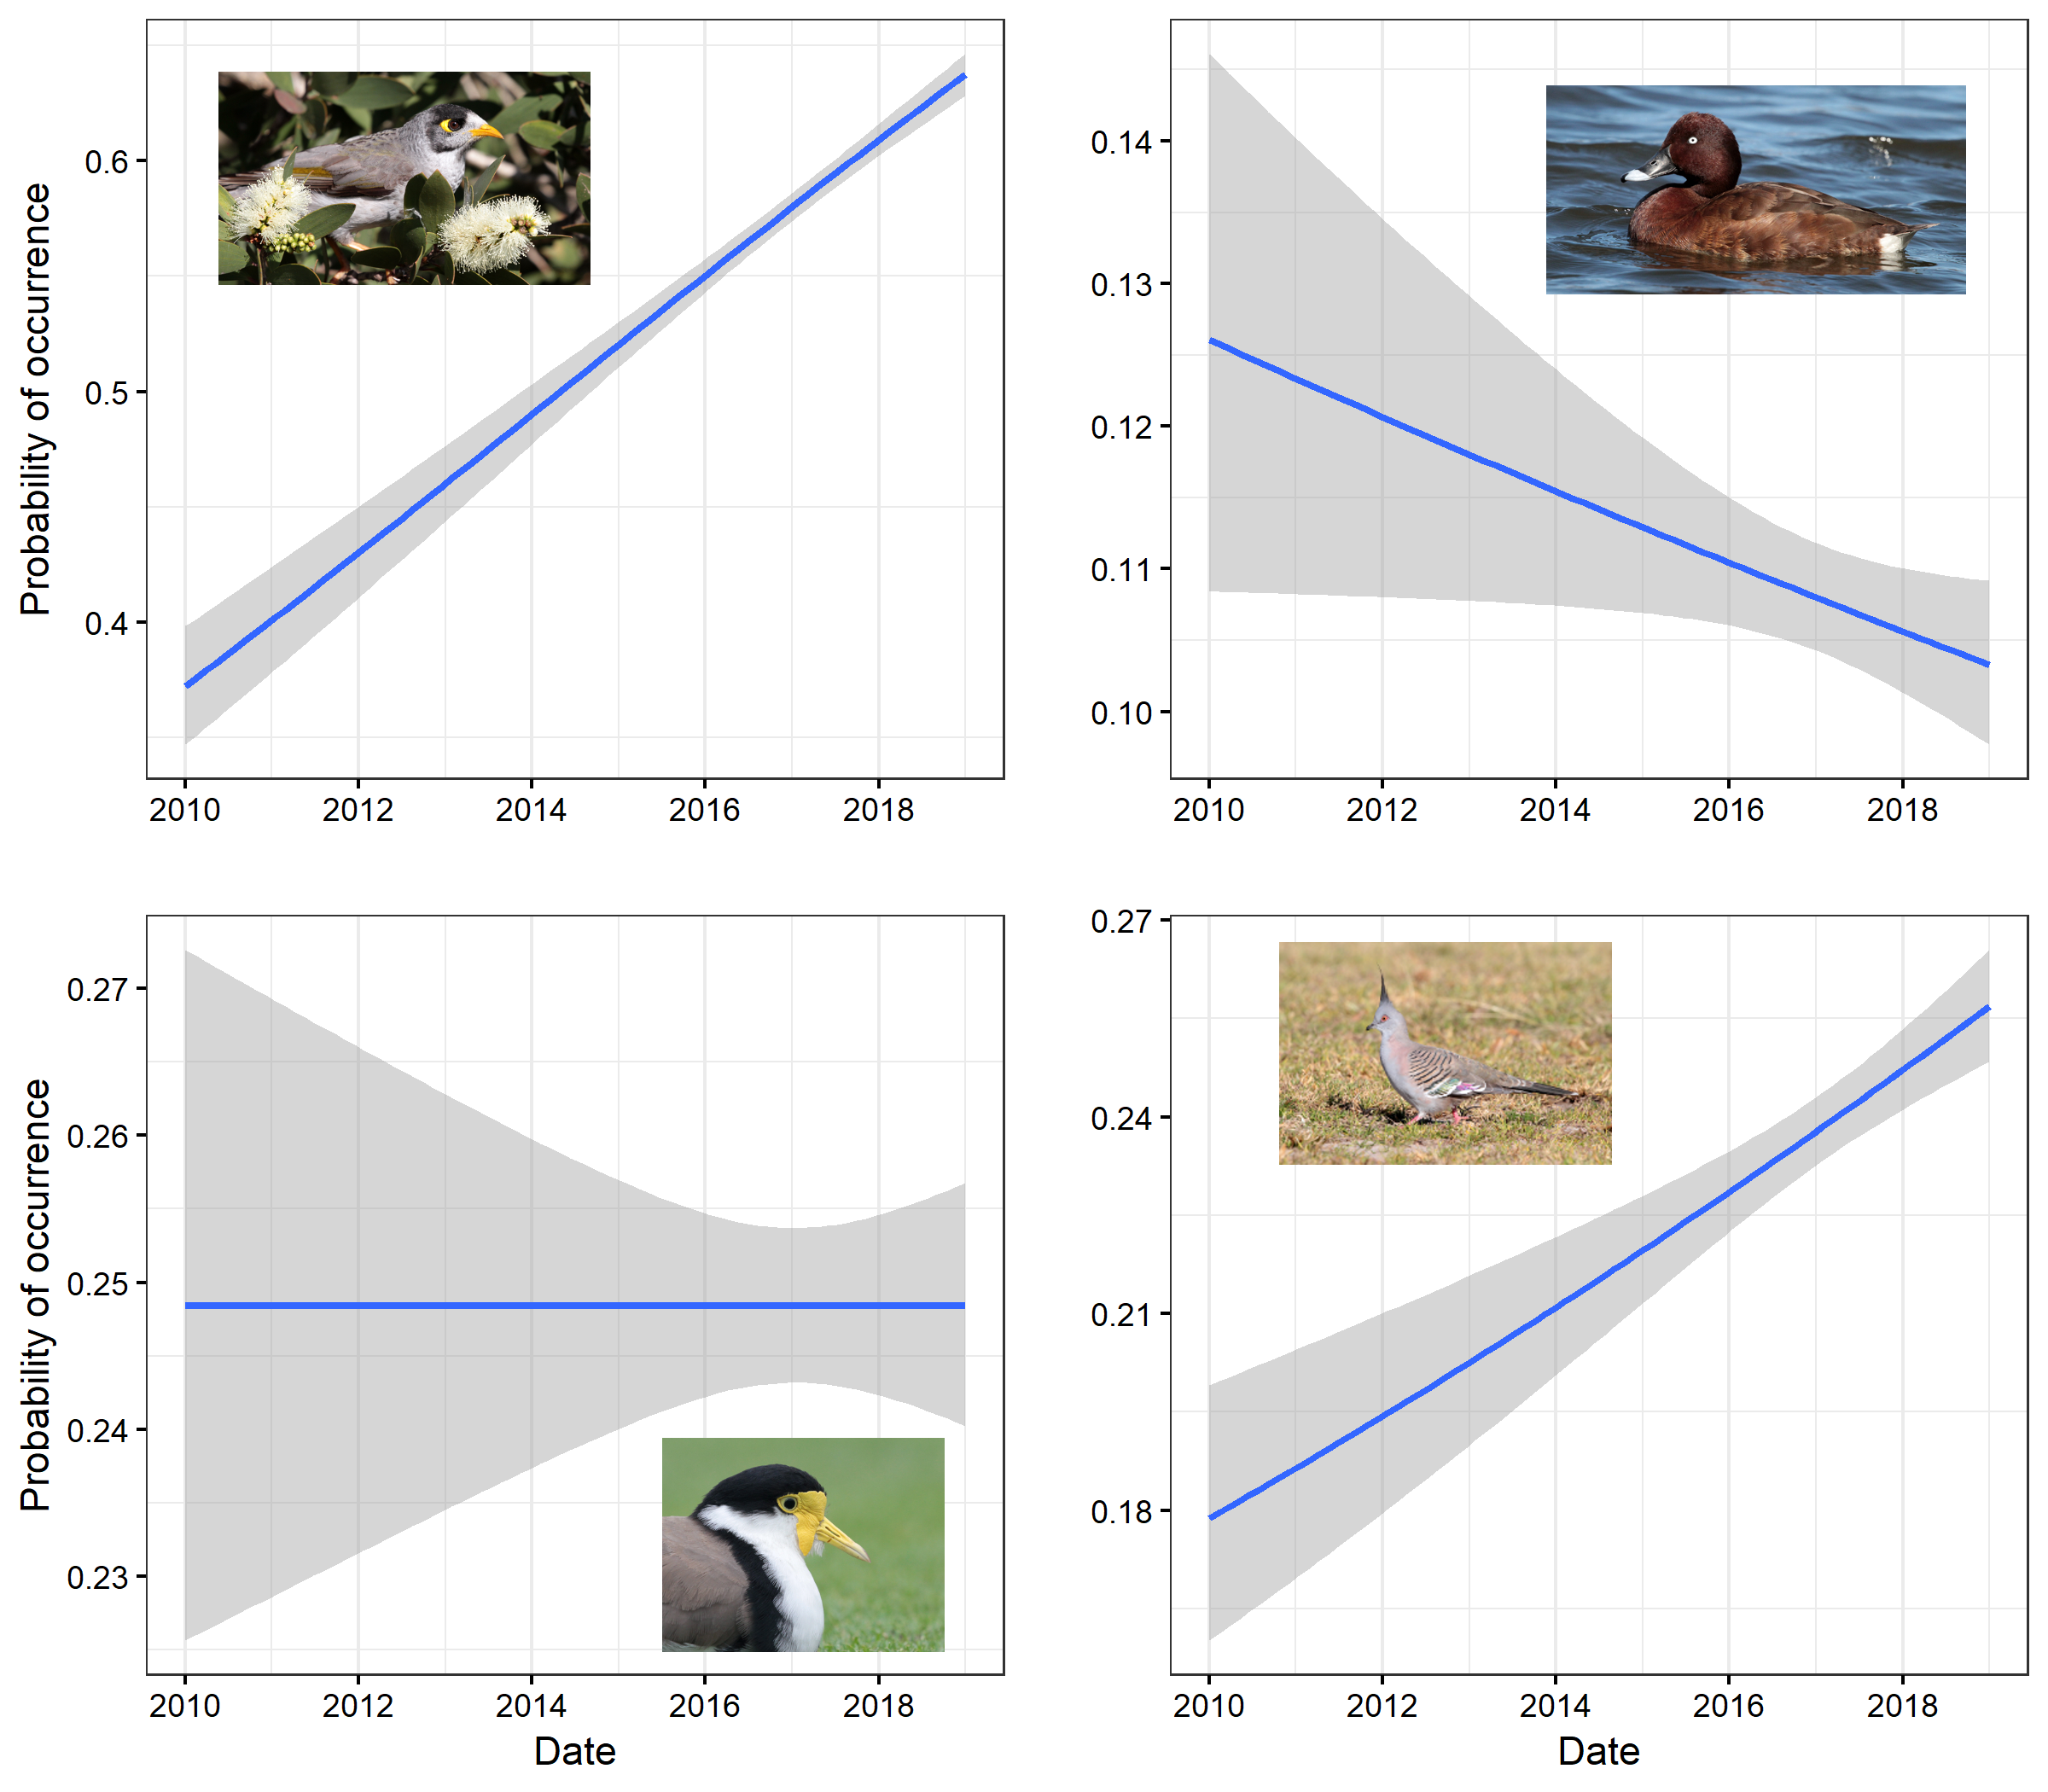
\includegraphics[width=.8\linewidth]{glm_examples_edited.png}
\caption{The ultimate goal in understanding population trends is to minimize the standard error for a population trend model, providing more robust measures of population trends. Shown here are four example population trend models, based on eBird data between 2010-2018, for Noisy Miner (top left), Hardhead (top right), Masked Lapwing (bottom left), and Crested Pigeon (bottom right).}
\label{fig1}
\end{figure}

The number of citizen science projects which are focused on ecological and environmental monitoring is increasing \cite{pocock2017diversity, theobald2015global}, highlighting the potential that citizen science holds for the future of ecology, conservation, and natural resource management \cite{pocock2018vision, silvertown2009new, soroye2018opportunistic, mckinley2017citizen}. But a major obstacle in the future use of citizen science data remains understanding how to best extract information from 'noisy' citizen science datasets \cite{parrish2018exposing}. As mentioned, this noise from citizen science \cite{bird2014statistical} can sometimes be alleviated using 'big-data' statistical approaches \cite{kelling2015taking}, but this is most applicable for data originating from large, successful citizen science projects --- with lots of data. What about projects that are just beginning? Or projects focusing on taxa that are less popular with the general public \cite{mair2016explaining, ward2014understanding}? Are there optimal strategies for sampling in space and time for estimating biodiversity trends?

Here, we investigate these questions with a specific objective: assess how spatial and temporal sampling influences trend detection of biodiversity. Our approach is dynamic: we are interested in the parameters that influence the marginal value of a given citizen science observation in both time and space. First, we summarize the parameters which we hyptohesized would influence the marginal value of a citizen science observation.

\subsection*{Predictions}

\begin{itemize}
  \item \textbf{Whether a site was sampled}: if a site had been previously sampled or not. We predicted that unsampled sites would be marginally more valuable than sampled previously sampled sites.
  \item \textbf{Median sampling interval}: the median of the distribution of waiting times between samples at a site. We predicted that the median sampling interval would be positively associated with the value of a citizen science observation. I.e., observations from sites with high median waiting times would be more valuable than observations from sites with low median waiting times.
  \item \textbf{Days since last sample}: the number of days between samples at a site. We predicted that the days since the last sample would positively associate with the value of a citizen science observation.
  \item \textbf{Distance to the nearest sampled site}: the distance between the site in question and the nearest sampled site. We hypothesized that for the distance to the nearest sampled site would be positively associated with the value of a citizen science observation.
  \item \textbf{Nearest neighbor sampling interval}: the median sampling interval of the nearest neighbor. We hypothesized that this would be positively influence the value of a observation, whereby well-sampled areas (i.e., multiple sites near each other with low median sampling intervals) would have lower value observations.
  \item \textbf{Number of unique days sampled}: the total number of unique days sampled for a given site. We predicted that the total number of unique days would be positively associated with the value of an observation, whereby sites with lots of observations would receive value given the long-term data originating from them.
\end{itemize}

We test our predictions using a popular citizen science project --- eBird \cite{sullivan2009ebird} --- and > 5 million bird observations from the Greater Sydney Region, NSW, Australia. We fit presence/absence population trend models to 235 species throughout this region, based on data from 2010 to 2018 (Fig. 1), and calculate statistical leverage for every citizen science sampling event, for each species. The leverage is a measure of how 'valuable' a given observation is to the population trend model for each species. Each sampling event is then assigned a cumulative measure of leverage --- i.e., marginal value. We then test our predictions above using linear models, assessing the influence each of the parameters has on the trend detection of biodiversity. Finally, we use the parameterized model results to predict the expected leverage (i.e., marginal value) for a given grid in space and time, producing a dynamic map of expected marginal value of citizen science sampling for every day in 2018.

\section*{Results and Discussion}
To assess the robustness of our approach, we investigated our predictions at four different grid sizes: 5, 10, 25, and 50 km$^{2}$ grids. We found weak evidence that visiting an unsampled grid was marginally more valuable than visiting an already sampled grid. There was no statistical significance for the 5 km (p=0.669), and 10 km (p=0.093) grid sizes, but there was for the 25 km (p=0.035) grid size. At the 50 km grid size, this test was not possible because all grids had been sampled. These results suggests that stratified sampling --- an approach which aims for equal sampling among grids or sites --- \cite{baillie2008toward, longino1997biodiversity} is not the most applicable approach for detecting trends using citizen science data. In other words, citizen scientists contributing to eBird, likely a large number who are qualified naturalists in their own right \cite{callaghan2018unnatural}, are already sufficiently sampling biodiversity in space.

\begin{figure}[!hb]
\centering
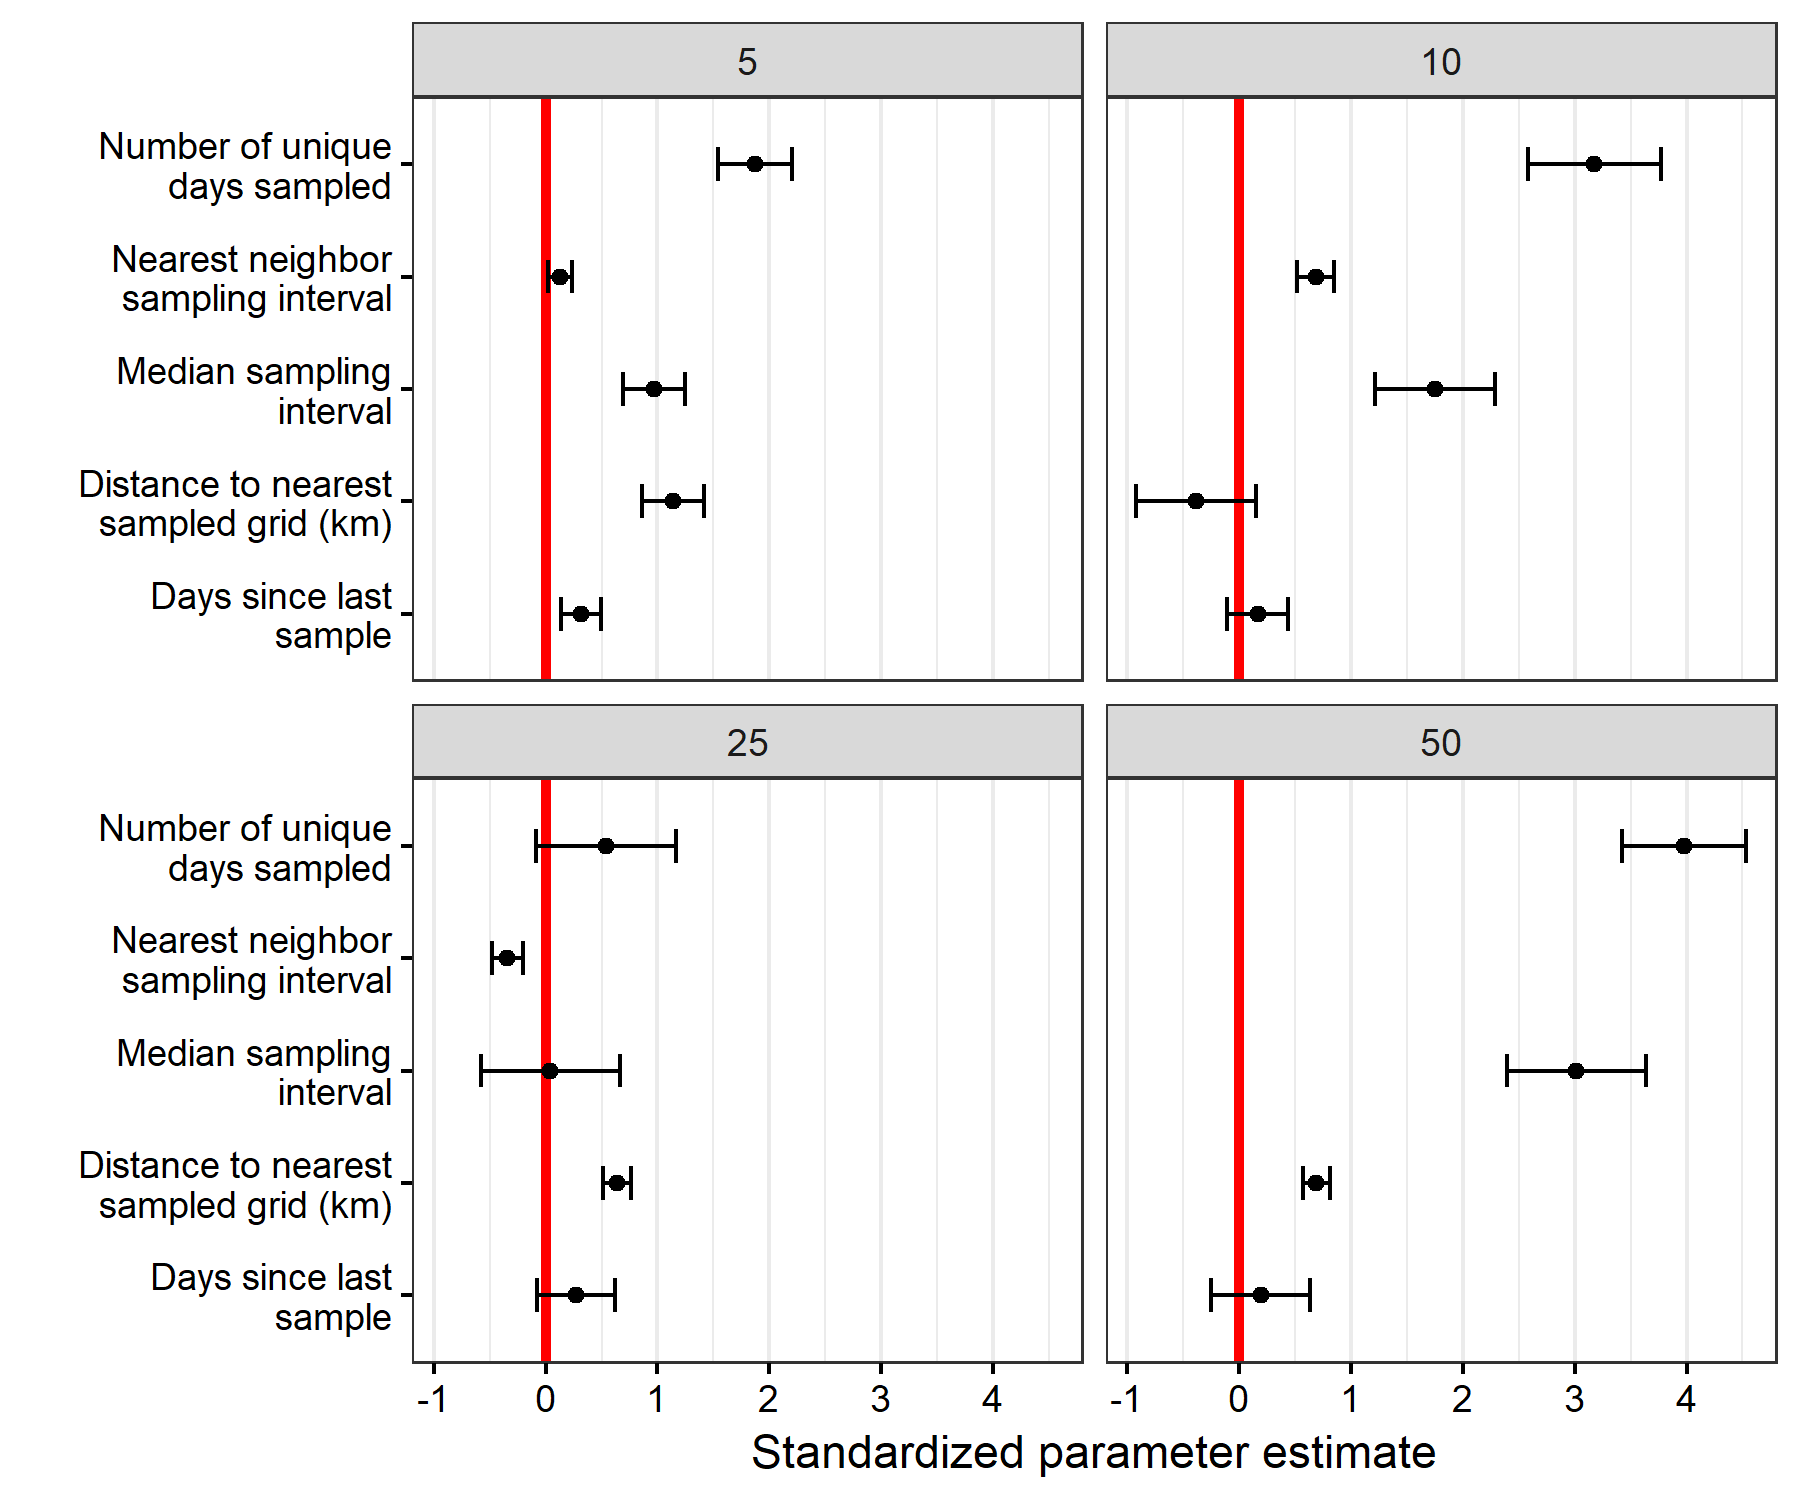
\includegraphics[width=.8\linewidth]{param_estimates.png}
\caption{Parameter estimates for standardized linear models for each of the four grid sizes (5, 10, 25, and 50). Variables were log-transformed and then standardized, allowing for the direct comparison among effect sizes.}
\label{fig2}
\end{figure}

For those sampled grids, however, we found significant relationships between a number of our predicted parameters and the marginal value of a sampling event (Fig. 2). In general, our parameters were positively associated with the marginal value of a sampling event. Of our parameters of interest, the number of unique days sampled (i.e., the `history' of a grid) had the strongest, positive, effect size, and this was robust to the grid size comparisons. The median sampling interval was also strongly associated with high marginal value samples, with an exception at the 25 km grid size. Distance to the nearest sampled grid and the nearest neighbor sampling interval influenced the marginal value of a sampling event less than the other parameters. Surprisingly, days since the last sample had less influence than the other parameters, albeit a positive association. The fact that days since last sample had a lower effect size than both the median sampling interval and the number of unique days sampled, likely highlights the value of `revisiting' a site in order to extract the maximum amount of information.

Together, these results suggest that there are possible improvements in biodiversity sampling for trend detection. In short, the `history' of a grid is important for considering whether to sample that grid: the number of unique days sampled was the strongest predictor, suggesting that observations from sites with a long time-series are marginally more valuable. Further, a secondary goal should be to decrease (i.e., left-shift the distribution) of the median sampling interval of the grids. The effect of number of days sampled was strongest at the largest grid size, suggesting that given all grids are sampled with some regularity --- as they are with larger grid sizes --- the importance of the `history' of a site is inflated.

We found generally consistent results, based on the grid size chosen, highlighting the robustness of spatial scale in our approach. It is critical to track biodiversity trends at multiple spatial scales \cite{soberon2007assessing}, as biodiversity estimates sometimes change dependent on the spatial scale \cite{chase2013scale}. Our approach of relying on statistical leverage as a measure of the value of a citizen science observation can be used regardless of whether a citizen science project is global, regional, or carried out in the constraints of a local park. In any instance, the area can be gridded --- the size of a grid, however, would be proportional to the spatial scale of the study --- and the framework implemented, updated dynamically.

Providing dynamic feedback to citizen science participants has proved successful for many citizen science projects \cite{rowley2019frogid, wiggins2011conservation, xue2016avicaching}. This feedback is generally in the form of leaderboards, presenting the number of submissions or number of unique species someone has contributed \cite{wood2011ebird}. We used our fitted models to predict the expected value of a given citizen science observation, dynamically, for any given day (e.g., Fig. 3, \href{https://github.com/coreytcallaghan/optimize_citizen_science_obs/blob/master/Figures/dynamic_map.gif}{Video S2}). This approach required us to look backward first, using a model with all observations for 2018, based on statistical leverage calculated from 2010-2018, in order to look forward and pedict the expected leverage for any given day. We envision a dynamic approach (Video S2) in the future of citizen science projects, which would ultimately guide participants to sites which \textit{should} be sampled on any given day --- or in a given week, month, or year. In this instance, leaderboards would move past numbers of species or submissions and complementary leaderboards could be derived based on a participant's cumulative value to the citizen science dataset, for biodiversity outcomes. Instead of participants preferrentially chasing specific species, this approach would guide participants to the sites with the highest expected marginal value. For example, we imagine visitor centers across the world at national parks or urban greenspaces providing their visitors on any given day a localized map showing which trail someone should visit if they are interested in contributing the greatest value to that park's biodiversity knowledge, through citizen science. The global pull of ecotourism \cite{sharpley2006ecotourism} is increasing exponentially, creating the potential for people to contribute to local biodiversity knowledge in areas that are traditionally undersampled, and with this framework, the collective effort of citizen scientists can be maximized.

\begin{figure}[!hb]
\centering
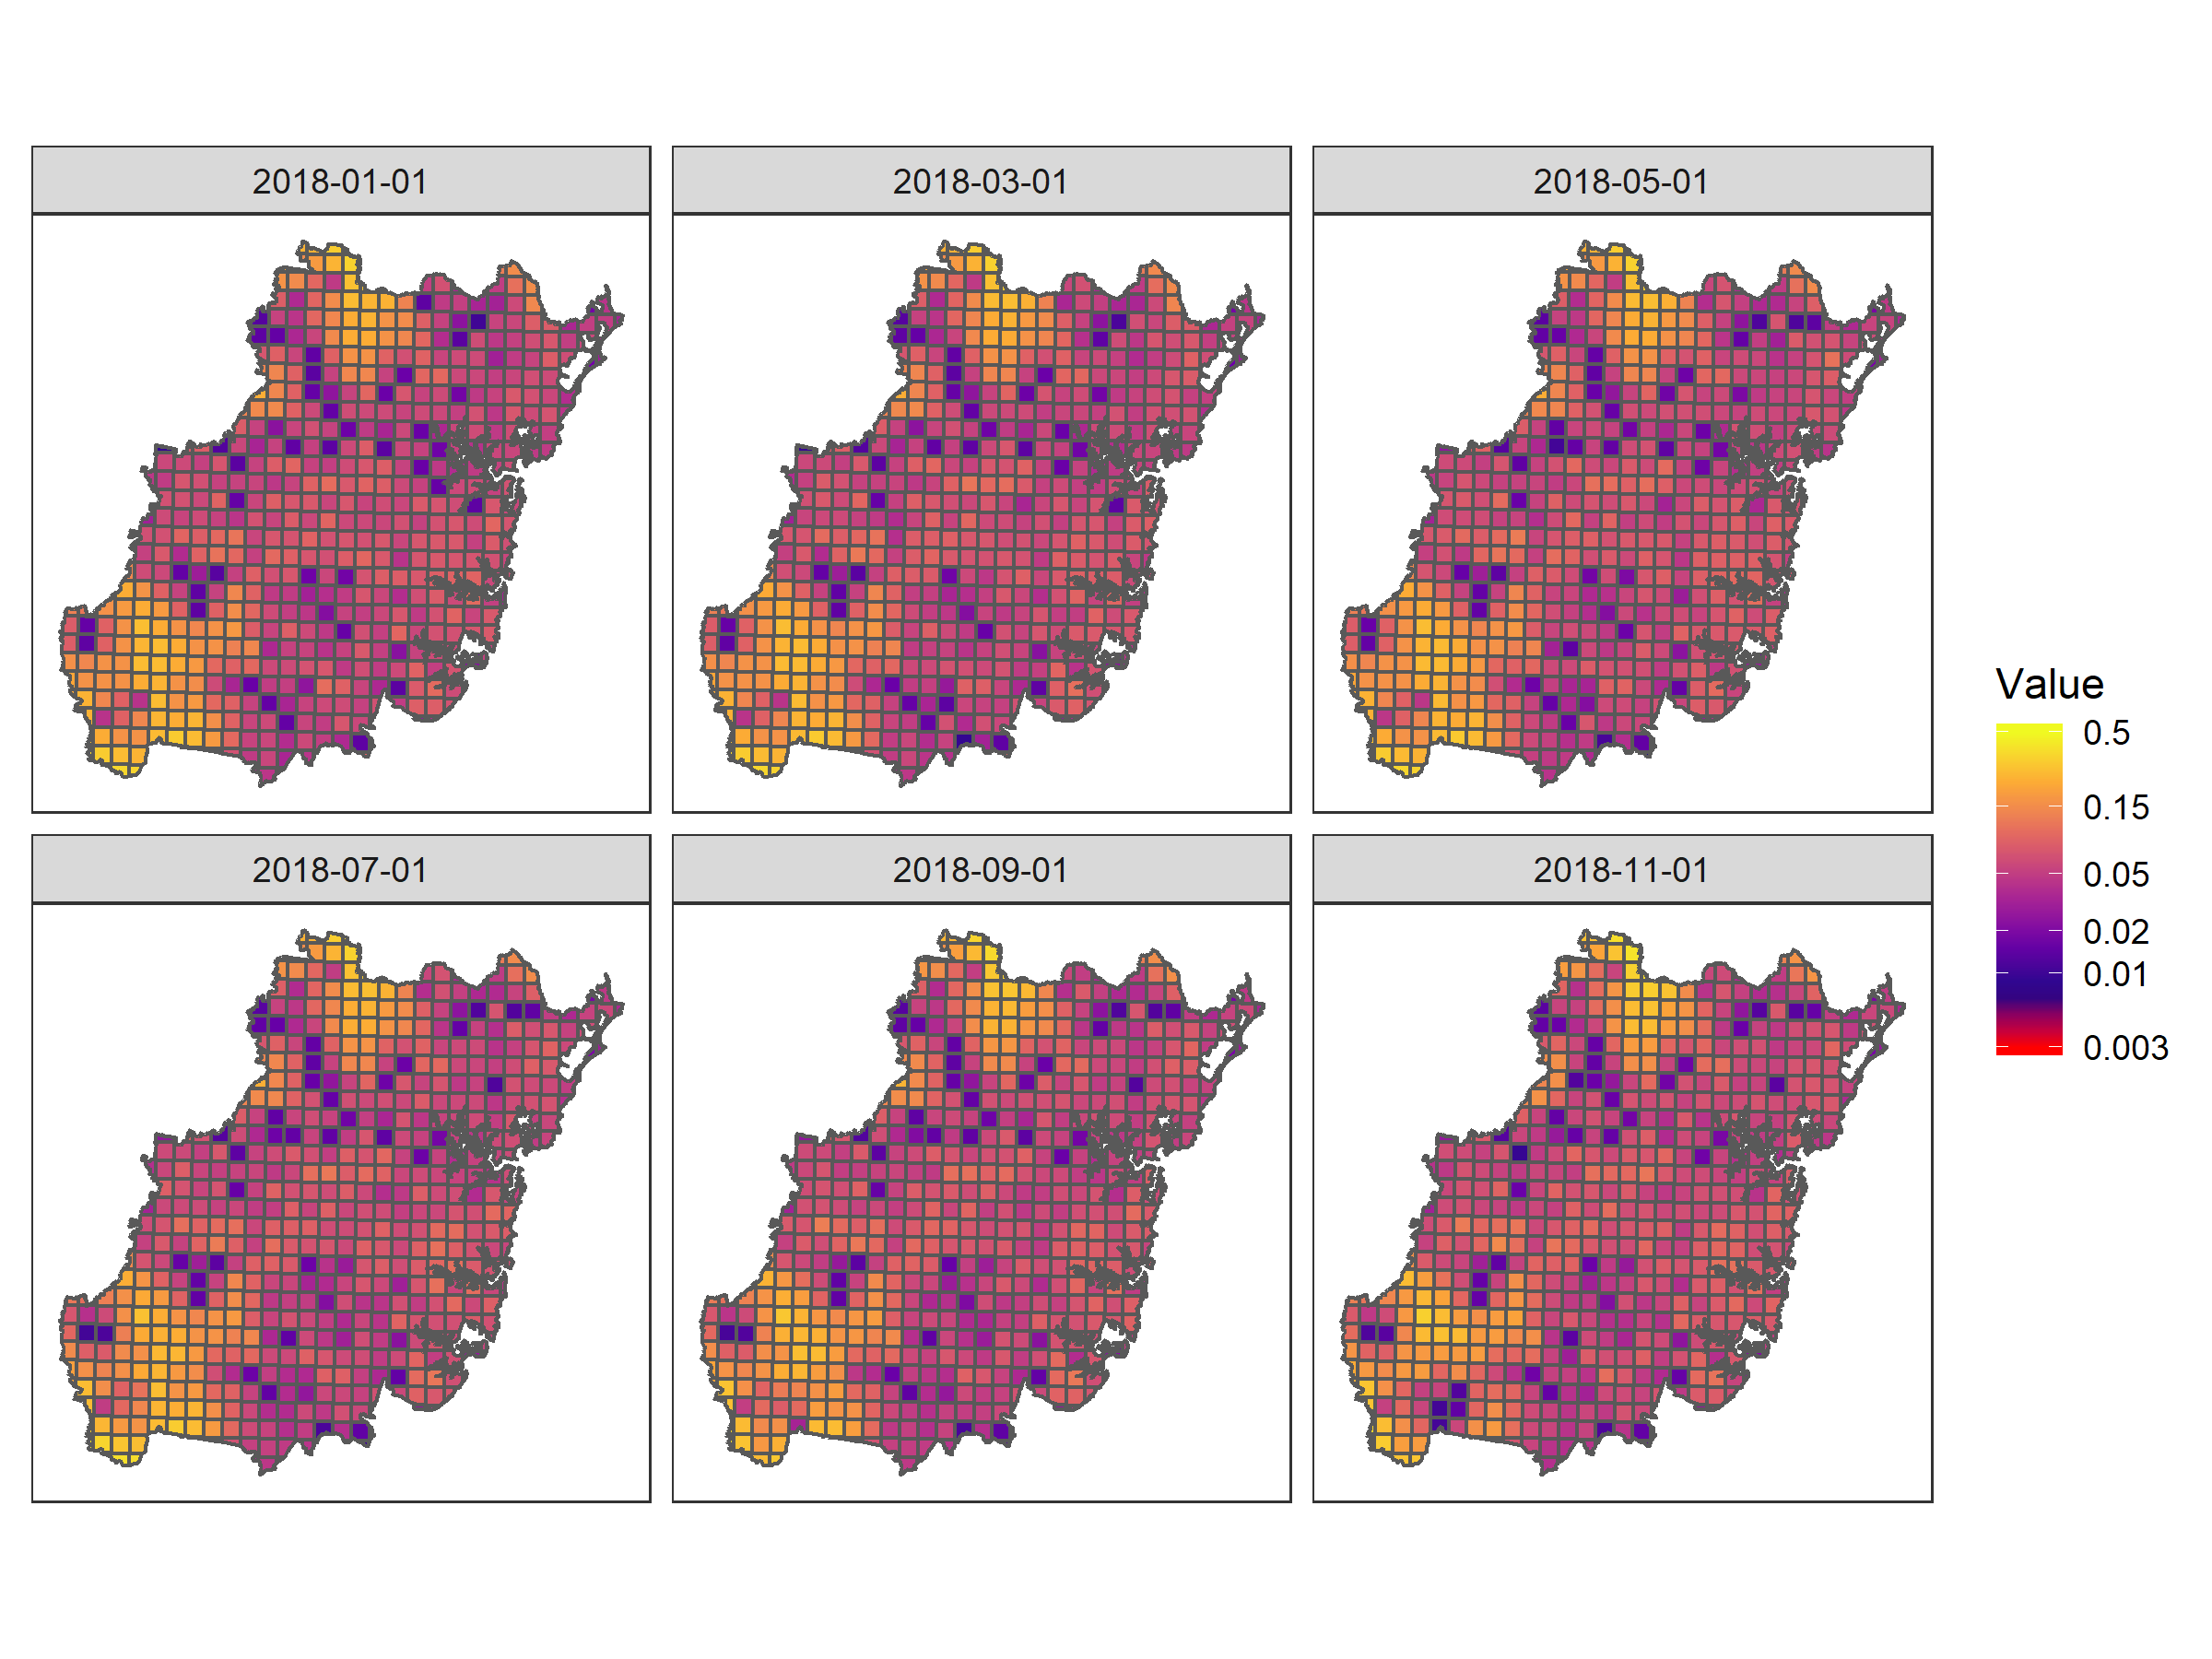
\includegraphics[width=.8\linewidth]{example_maps.png}
\caption{A map of predicted expected marginal value for six different days in 2018, throughout the Greater Sydney Region, showing the highest valued grid cells that would optimize the collective knowledge on biodiversity trends throughout the Greater Sydney Region. This is a dynamic approach, where the predictions are updated as new observations are submitted to the citizen science database, and we have done this for every day in 2018 (\href{https://github.com/coreytcallaghan/optimize_citizen_science_obs/blob/master/Figures/dynamic_map.gif}{Video S2}).}
\label{fig3}
\end{figure}

We focused our framework on a specific statistical outcome: trend detection. Many other ecological outcomes arise from citizen science datasets, including species distribution models \cite{bradsworth2017species, van2013opportunistic}, phylogeographical research \cite{bahls2014new, drury2019continent}, invasive species detection \cite{pocock2017citizen, grason2018citizen}, or phenological research \cite{la2014role, supp2015citizen}. Each potential outcome will have different optimal sampling strategies in space and time, likely with nuanced trade-offs between outcomes. But these different outcomes can still be quantified in the same framework we introduce here. For example, an intended outcome of a spcecies distribution model would likely place greater value on observations from unsampled grids \cite{crawley2001scale} than for species trend detection. Our framework is robust, with the necessary piece of information being a statistical model based on an intended ecological/management outcome.

\subsection*{Conclusions}
Since eBird's inception in 2002, citizen scientists have collectively contributed > 30 million effort hours. And this is only one citizen science project. Clearly, the cumulative effort put-forth by citizen scientists is immense, and arguably, citizen science will continue to shape the future of ecology and conservation --- as it has substantially for the past couple centuries \cite{silvertown2009new} --- with an increasingly critical role \cite{mckinley2017citizen, pocock2018vision} in monitoring of biodiversity. But we need to look towards the future. Are there mechanisms we can put in place now which will increase our collective knowledge gleaned from citizen science datasets for biodiversity in the future? We highlighted general rules which could help to guide citizen science participants to better sampling in space and time: the number of unique days sampled and the largest median sampling intervals both positively correlate with the marginal value of a citizen science observation. Moreover, we demonstrate a framework which practicioners can implement to better optimize their sampling designs, specific to a citizen science project and an intended goal.

\matmethods{ We tested our predictions throughout the Greater Sydney Region, delineating grids across the region of varying size: 5, 10, 25, and 50 km$^{2}$, where a grid represented a 'site'. We used the R statistical environment \cite{rcoreteam2018r} to carry out all analyses, relying heavily on the tidyverse \cite{wickham2017tidyverse}, ggplot2 \cite{wickham2016ggplot}, and sf \cite{pebesma2018sf} packages.

In order to test our predictions, we used the eBird basic dataset (version $ebd-relDec-2018$; available at: https://ebird.org/data/download), subsetting the data between January 1$^{st}$, 2010 and December 31$^{st}$, 2018. eBird is a particularly successful citizen science project with > 600 million observations contributed by > 400 thousand participants, globally \cite{sullivan2009ebird, sullivan2014ebird, sullivan2017using}. eBird relies on volunteer birdwatchers who collect data in the form of 'checklists' --- a list of all species identified (audibly or visually) for given spatiotemporal coordinates. eBird relies on an extensive network of regional reviewers who are local experts of the avifauna \cite{gilfedder2019brokering} to ensure data quality \cite{sullivan2009ebird}.

\subsection*{Trend detection model} We first filtered the eBird basic dataset \cite{callaghan2017assessing, johnston2018estimates, la2014role}, by the following criteria: (1) we only included complete checklists, (2) only included terrestrial bird species, (3) removed any nocturnal checklists, (4) only included checklists which were > 5 minutes and < 240 minutes in duration, (5) only included checklists which travelled < 5 km or covered < 500 Ha, and (6) only included checklists which had > 4 species on it, as checklists with less than 4 species were likely to be targeted searches for particular species \cite{walker2017using, szabo2010regional}.

For any species with > 50 observations (N=235), we fit a generalized linear model using the 'glm' function in R, based on presence/absence \cite{walker2017using, horns2018using}. The models consisted of a continuous term for day, beginning January 1$^{st}$, 2010, and a categorical term for county, providing a spatial component to the models (e.g., Fig. 1). We also included an offset term for the number of species seen on a given eBird checklist, accounting for temporal and spatial effort of that checklist \cite{szabo2010regional}. Each of the models were fit with a binomial family distribution. A total of 25,995 observations (i.e., eBird checklists) were used to fit each of the models.

\subsection*{Statistical leverage} Statistical leverage measures the influence of a particular observation on the independent variable \cite{cook1977detection}. In other words, it is a measure of how much a given observation influences the results of a statistical outcome. In our instance, we had multiple predictor variables in our GLMs, and so we used dfBeta as a measure of statistical leverage for each observation. dfBeta measures the change to the observed parameters of a new regression equation, after omitting the \textit{i$^{th}$} observation from the dataset \cite{belsley1980regression}. It follows the formula:

\begin{equation}
D F B E T A=\hat{\beta}-\beta_{(i)}=\frac{\left(X^{\prime} X\right)^{-1} X_{i} r_{i}}{1-h_{i}}
\end{equation}

where X is the predictor variable matrix, \textit{r} the residual vector, \textit{i h} the \textit{i$^{th}$} diagonal member, and \textit{i x} the \textit{i$^{th}$} line of matrix X. The value of dfBeta proportionally decreases with increasing number of observations.

In our case, each observation for a given species recieved a dfBeta value (i.e., each species received 25,995 measures of dfBeta), using the 'dfbetas' function from R \cite{rcoreteam2018r}. The measure of statistical leverage, then, of a given checklist was the sum of the absolute value of the dfBeta measures for each species (i.e., the sum of all 235 dfBetas). This measure of statistical leverage was thus a measure of a checklist's influence in understanding cumulative species' trends throughout the Greater Sydney Region, and accordingly represented the marginal value of that particular checklist.

\subsection*{Parameter calculation} After our model was fit from 2010---2018, we calculated the predicted parameters of interest for each day in 2018 (N=365). For each individual grid, at each of the grid sizes, we dynamically calculated the following parameters: (1) whether a grid cell had ever been sampled, (2) the distance to the nearest sampled grid cell, (3) the median sampling interval of a grid cell, (4) the median sampling interval of the nearest sampled grid cell, (5) days since the last sample in a grid cell, and (6) the duration of sampling in a grid cell --- most recent sample minus the earliest sampled date, and (7) the number of unique sampling days within the grid cell.

We then subsetted the leverage calculations (see above) for each of the days in 2018, given we know where people sampled, relative to the parameters for each of the grids on that day. We ran a linear regression, for each of the different grid sizes considered in the analysis, to investigate what parameters were of significant interest. Prior to modelling, duration was highly correlated with median sampling interval for the majority of the grid size analyses, and as such, was excluded from consdieration. Given the paramters' correlation varied among grid cell sizes, we needed to ensure a robust, and simple model. All variables were log-transformed and then standardized prior to modelling, ensuring that the effect sizes of the given parameters were meaningful. The response variable, dfBeta (i.e., value) was log-transformed prior to modelling to meet model assumptions. Thus, the final model included a log-tranformed dfBeta response variable, regressed against log-transformed standardized median sampling interval, number of days sampled, days since the last sample, distance to the nearest sampled neighbor, and the neighbor's median sampling interval.

After our model was fit, we used the 'augment' function from the broom package \cite{robinson2018broom} to predict the expected leverage for every grid cell in the Greater Sydney Region, for every day. For grid cells which were unsampled, we assigned them the mean of the sampled grid cells, based on our lack of evidence that unsampled cells were significantly more valuable than sampled cells. Where one grid had multiple predicted leverages (i.e., where a grid had more than one checklist in a day), we randomly sampled to one of these expected leverages. This prediction process was repeated for every day of 2018.

\subsection*{Data availability} All eBird data are freely available for download (https://ebird.org/data/download), but the necessary portion of the eBird basic dataset, along with spatial data, and code to reproduce our analyses are available at: https://github.com/coreytcallaghan/optimize_citizen_science_obs.
}

\showmatmethods{} % Display the Materials and Methods section

\acknow{We thank the countless citizen scientists who are contributing data that is continuously increasing our collective knowledge of biodiversity.}

\showacknow{} % Display the acknowledgments section

% Bibliography
\bibliography{refs}

\end{document}
